\chapter{Low numeric convolution neural network}
\label{ch:low prec NN}
\textcolor{purple}{What knowledge is necessary to}
\begin{itemize}
    \item \textcolor{purple}{understand design decisions you made, e.g. how did you choose the quantisation algorithm?}
    \item \textcolor{purple}{understand why your research question is important, e.g. why should we quantise CNNs?}
\end{itemize}
In this chapter, we go through the basic of convolution neural network, the mindset behind choosing linear quantization scheme, an algorithm for training a ultra-low precision neural network on large-scale dataset and finally a tensor re-pack method for deploying the network on a processor supporting low-precision MAC operation.
\section{Convolutional Neural Networks}
A typical convolution neural network layer takes a 3D \textit{input tensor} and a \textit{filter tensor}, and performs 2D convolution, producing a 3D \textit{output tensor}.It is essentially summing up \textbf{C} channel of 2D convolution for one output pixel as shown in \autoref{fig:conv_1}, this process is repeated for \textbf{M} number of filter, resulting output tensor of \textbf{M} number of channel. 
In \autoref{fig:conv_2} shows a common techniques \textit{batching}, taking multiple input tensor and perform convolution on them at the same time; the picture also provides an example of the shape parameter \textbf{U}.
\begin{figure}[h]
    \centering
    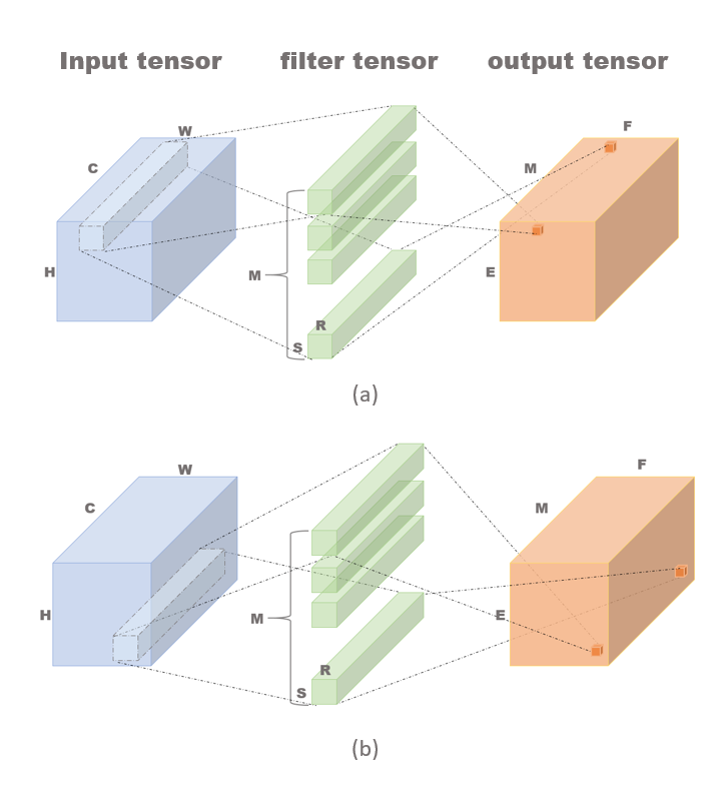
\includegraphics[width=1\linewidth]{inc/3_low_numeric_convolution_neural_network/figure/convolution_1.png}
    \caption{Computation of a convolutional layer.}
    \label{fig:conv_1}
\end{figure}
\begin{figure}[h]
    \centering
    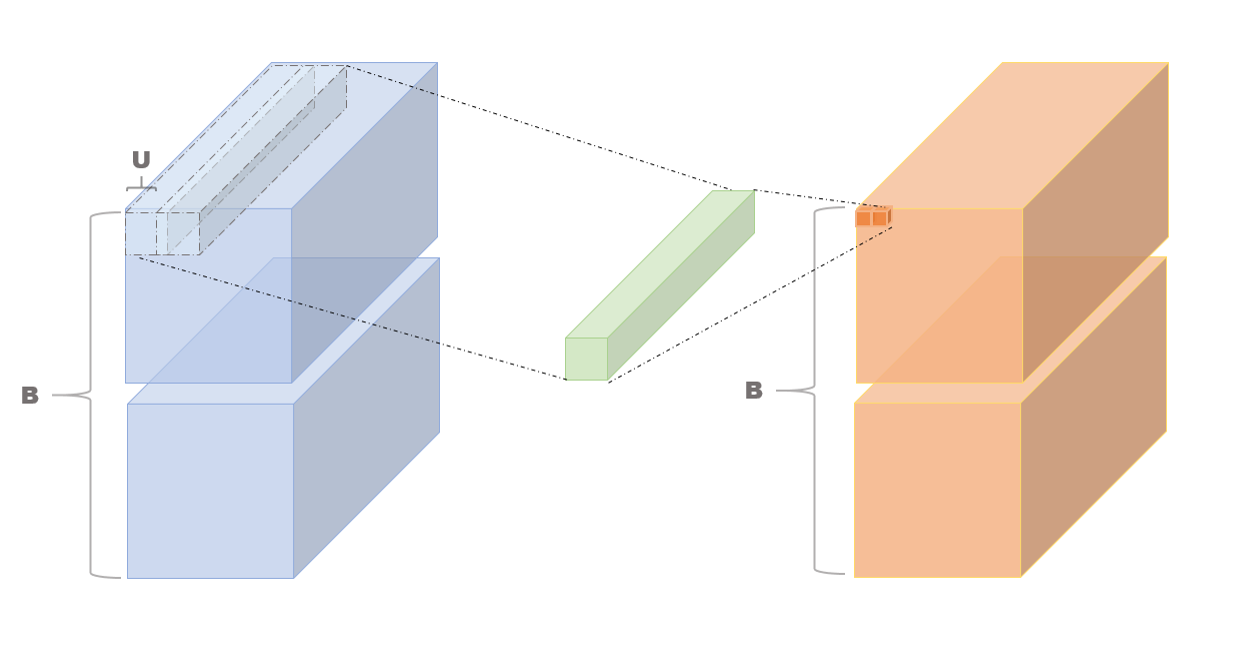
\includegraphics[width=1\linewidth]{inc/3_low_numeric_convolution_neural_network/figure/convolution_2.png}
    \caption{Shape parameter B and U.}
    \label{fig:conv_2}
\end{figure}
The entire process is formulated by \autoref{eq:conv}:
\begin{equation}
    \begin{aligned}\label{eq:conv}
    \boldsymbol{O}[z][u][x][y]=\text{ReLU}\,(
        \sum^{C-1}_{k=0}\sum^{R-1}_{i=0}\sum^{S-1}_{j=0}\boldsymbol{I}[z][k][Ux+i][Uy+j]*\boldsymbol{W}[u][k][i][j]
    ), \\
    0\leq z\leq B\ , 0\leq u\leq M\ , 0\leq y\leq E\ , 0\leq x\leq F, \\
    E=(H-R+U)/U,\,F=(W-S+U)/U
    \end{aligned}
\end{equation}


\begin{table}
    \caption{Basic shape parameters of a CNN layer.}
    \label{tab:cnn_shape}
    \centering
    \footnotesize 
        \begin{tabular}{cc}
        \toprule
        Parameter & Description \\
        \midrule
        H/W & Input feature map spatial dimensions\\
        E/F & Output feature map spatial dimensions\\
        R/S & Filter spatial dimensions\\
        C & Input channels\\
        M & Output filters\\
        U & stride\\
        B & Batch,\# of feature maps to be processed\\
        \bottomrule
        \end{tabular}
\end{table}


 
\section{Low Precision CNN}
\section{Reconstruction Loss Minimization Thresold Selection}
\section{Computational consideration and data re-packing}

\begin{table}
    \caption{Tiling shape parameters.}
    \label{tab:tile_shape}
    \centering
    \footnotesize 
        \begin{tabular}{cc}
        \toprule
        Parameter & Description \\
        \midrule
            $T_m$ & filters\\
            $T_w$ & feature map Width tile\\
            $T_h$ & feature map Height tile\\
            $T_b$ & Batch tile\\
        \bottomrule
        \end{tabular}
\end{table}

\begin{table}
    \caption{Low bit arithmetic and shape parameters.}
    \label{tab:bit_shape}
    \centering
    \footnotesize 
        \begin{tabular}{cc}
        \toprule
        Parameter & Description \\
        \midrule
        $X_b$ & Input bit channels\\
        $W_b$ & Weight bit channels\\
        $O_b$ & Output bit channels\\
        $A_b$ & Arithmetic bit length\\
        \bottomrule
        \end{tabular}
\end{table}
\begin{table}
    \caption{PE processing shape parameters.}
    \label{tab:pe_shape}
    \centering
    \footnotesize 
        \begin{tabular}{cc}
        \toprule
        Parameter & Description \\
        \midrule
        $P_m$ & Filters in a PE\\
        $P_{ch}$ & Channels in a PE\\
        \bottomrule
        \end{tabular}
\end{table}